% ******************************************************** %
%              TEMPLATE DE INFORME ORGA2 v0.1              %
% ******************************************************** %
% ******************************************************** %
%                                                          %
% ALGUNOS PAQUETES REQUERIDOS (EN UBUNTU):                 %
% ========================================
%                                                          %
% texlive-latex-base                                       %
% texlive-latex-recommended                                %
% texlive-fonts-recommended                                %
% texlive-latex-extra?                                     %
% texlive-lang-spanish (en ubuntu 13.10)                   %
% ******************************************************** %


\documentclass[a4paper]{article}
\usepackage[spanish]{babel}
\usepackage[utf8]{inputenc}
\usepackage{charter}
\usepackage{lipsum}
\usepackage{subfig}
% tipografia
\usepackage{graphicx}
%\usepackage{makeidx}
\usepackage{paralist} %itemize inline
%\usepackage{float}
%\usepackage{amsmath, amsthm, amssymb}
%\usepackage{amsfonts}
%\usepackage{sectsty}
%\usepackage{charter}
%\usepackage{wrapfig}
%\usepackage{listings}
%\lstset{language=C}
\usepackage{wrapfig}

% \setcounter{secnumdepth}{2}
\usepackage{underscore}
\usepackage{caratula}
\usepackage{url}


% ********************************************************* %
% ~~~~~~~~              Code snippets             ~~~~~~~~~ %
% ********************************************************* %

\usepackage{color} % para snipets de codigo coloreados
\usepackage{fancybox}  % para el sbox de los snipets de codigo

\definecolor{litegrey}{gray}{0.94}

\newenvironment{codesnippet}{%
	\begin{Sbox}\begin{minipage}{\textwidth}\sffamily\small}%
	{\end{minipage}\end{Sbox}%
		\begin{center}%
		\vspace{-0.4cm}\colorbox{litegrey}{\TheSbox}\end{center}\vspace{0.3cm}}



% ********************************************************* %
% ~~~~~~~~         Formato de las páginas         ~~~~~~~~~ %
% ********************************************************* %

\usepackage{fancyhdr}
\pagestyle{fancy}

%\renewcommand{\chaptermark}[1]{\markboth{#1}{}}
\renewcommand{\sectionmark}[1]{\markright{\thesection\ - #1}}

\fancyhf{}

\fancyhead[LO]{Sección \rightmark} % \thesection\ 
\fancyfoot[LO]{\small{Luis Ricardo Bustamante, David Alejandro Venegas Ramírez}}
\fancyfoot[RO]{\thepage}
\renewcommand{\headrulewidth}{0.5pt}
\renewcommand{\footrulewidth}{0.5pt}
\setlength{\hoffset}{-0.8in}
\setlength{\textwidth}{16cm}
%\setlength{\hoffset}{-1.1cm}
%\setlength{\textwidth}{16cm}
\setlength{\headsep}{0.5cm}
\setlength{\textheight}{25cm}
\setlength{\voffset}{-0.7in}
\setlength{\headwidth}{\textwidth}
\setlength{\headheight}{13.1pt}

\renewcommand{\baselinestretch}{1.1}  % line spacing

% ******************************************************** %

\usepackage{lipsum}
\usepackage{courier}


\begin{document}


\thispagestyle{empty}
\materia{Organización del Computador II}
\submateria{Primer Cuatrimestre de 2020}
\titulo{Trabajo Práctico II}
\subtitulo{Filtros en SIMD}
\integrante{Venegas Ramírez, David Alejandro}{783/18}{davidalevng@gmail.com}
\integrante{Bustamante, Luis Ricardo}{43/18}{luisbustamante097@gmail.com}

\maketitle
\newpage

\thispagestyle{empty}
\vfill
\begin{abstract}

En el presente trabajo se describe la problemática de implementar filtros para imágenes de manera eficiente utilizando SIMD, así como un análisis comparativo entre diferentes niveles de optimización en los compiladores de C versus el código en lenguaje ensamblador. Por último se busca contrastar diferentes versiones del código en SIMD a fin de plantear hipótesis sobre el rendimiento de diferentes implementaciones  y comprobar los beneficios de estas mediante la experimentación.

\end{abstract}

\thispagestyle{empty}
\vspace{3cm}
\tableofcontents
\newpage


%\normalsize
\newpage

\section{Introducción}

El objetivo de este trabajo práctico es implementar los contenidos vistos en las clases de Organización del Computador 2 y desarrollar filtros para imágenes utilizando el set de instrucciones \textbf{Streaming SIMD Extensions (SSE)} de la arquitectura intel-x86 donde SIMD es el modelo de cómputo \emph{Single Instruction, Multiple Data} para operar de forma paralela sobre los valores de los píxeles optimizando el performance, disminuyendo la cantidad de instrucciones necesarias y los saltos en el procesador así como el tiempo de cómputo. 

Durante el presente proyecto se desarrollan filtros para imágenes de formato BMP por su simplicidad y facilidad de uso, estas tienen un encabezado y un mapa de bits que representa la información de los píxeles. Se utilizan las bibliotecas proporcionadas por la cátedra de forma que cada filtro trabaja sobre un puntero al source o inicio de la matriz de píxeles. Donde cada celda tiene las componentes azul (B), verde (G) y rojo (R), y alpha(A). Cada componente se representa con 8 bits (1 byte) y valores sin signo dentro del rango [0, 255], excepto por la componente de transparencia (A) o alpha donde el valor siempre debe ser 255.

Ante todo, los filtros deben ser eficientes en recursos y operar en paralelo, razón por la cual se trabaja de a 4 píxeles por iteración en cada implementación mediante el uso de instrucciones SSE. Estos filtros se dividen en: \textbf{Ocultar, Descubrir y ZigZag}. El primero toma un puntero a imagen pasado como parámetro y esconde el archivo dentro de otra imagen también recibida mediante un puntero, esto lo logra primero reduciendo el tamaño de la imagen a ocultar convirtiéndola a escala de grises y luego guardando la información en los bits menos significativos de las imagen contenedora. Por ultimo se usa un algoritmo de confusión que dificulta la extracción posterior de la imagen, de forma que solo sea extraída con facilidad utilizando el filtro de Descubrir. Este otro filtro como su nombre lo indica extrae la imagen en escala de grises de una imagen contenedora donde ya fue aplicado el filtro Ocultar anteriormente (con el algoritmo correcto de confusión); este proceso se conoce como estenografía.  Por último, está el filtro de ZigZag que no tiene efectos prácticos para el espionaje pero sí genera una curiosa modificación estética en la imagen con un efecto de zigzag.

Por último, se realizan experimentos para comprobar la eficacia del código en assembly x86 usando SIMD vs. diferentes optimizaciones del compilador y diferentes compiladores, así como comparaciones entre diferentes implementaciones a fin de obtener una apreciación empírica sobre el rendimiento de los filtros y el set de instrucciones elegidas para desarrollarlos. 

\section{Desarrollo}

En el desarrollo de este trabajo práctico se contó con un framework provisto por la cátedra con todo lo necesario para poder leer y escribir imágenes, ası como también compilar y probar las funciones a implementar.

\subsection{Filtro Ocultar} \label{sec:filtro-ocultar}

El filtro Ocultar toma una imagen A y una imagen B como entrada, y devuelve una imagen A modificada, visualmente exacta a la original, pero con la imagen B en escala de grises oculta dentro de los bits menos significativos de cada píxel de la imagen resultado, con la particularidad de que los bits menos significativos están conformados como se muestra en la Figura \ref{fig:filtro-ocultar-bits}. Nótese que $src$ representa a la imagen A, $src2$ representa a la imagen B y $src(mirror)$ representa a los píxeles espejo de la imagen A, es decir, los píxeles que tomaría si se recorriera la imagen desde la esquina inferior derecha. Por ultimo la imagen resultado se la muestra como $dst$.

\begin{figure}[h]
  \begin{center}
	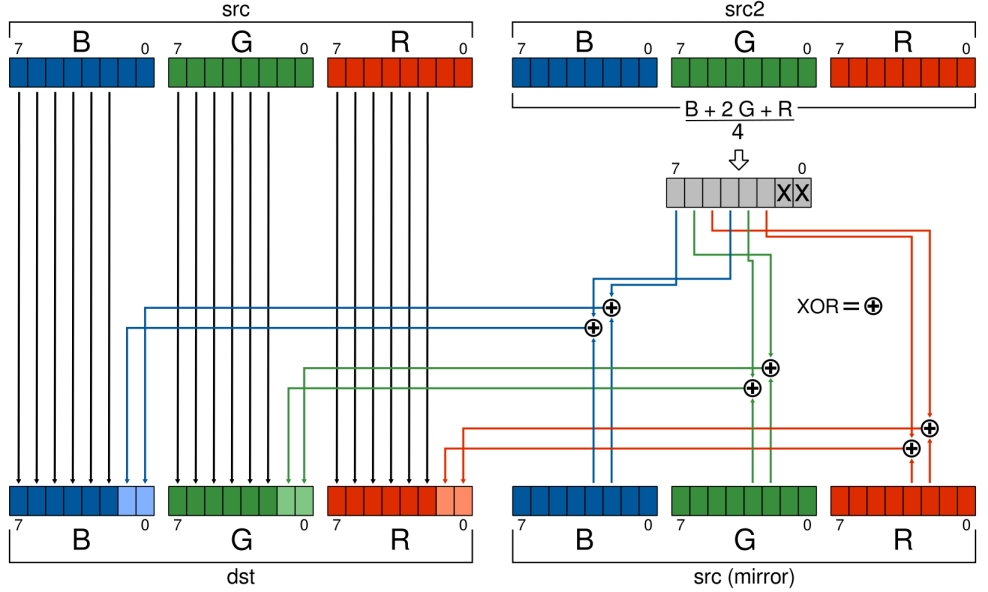
\includegraphics[scale=0.30]{images/filtro-ocultar-bits.jpg}
	\caption{Proceso completo de como funciona el filtro Ocultar}
	\label{fig:filtro-ocultar-bits}
  \end{center}
\end{figure}

\newpage
 
\subsubsection{Implementación en ASM}
 

La implementación de este filtro es un tanto complicada por el manejo de bits que se va a hacer al ocultar los bits de los píxeles de la imagen B (llamada $src2$ de ahora mas) dentro de la imagen A (llamada $src$ de ahora en mas). El proceso se divide en 3 partes: primero el conseguir los píxeles en escala de grises del $src2$, luego el reacomodar los píxeles conseguidos de la manera que se muestra en la Figura \ref{fig:filtro-ocultar-bits}, para finalmente poder mergearlos (mediante la instruccion PXOR) con los bits 2 y 3 del $src(mirror)$ y volcarlos en la imagen resultado (llamada $dst$). Además cabe destacar que el filtro opera con 4 píxeles a la vez, ya que cada píxel contiene 4 componentes las cuales tienen un tamaño de 1B cada uno, por lo que se puede operar de a 4 píxeles en total en un registro XMM. Este ultimo detalle puede no ser representado en alguna de las figuras que se presente a lo largo de esta sección, pero no significa que se haya dejado de trabajar con 4 píxeles a la vez.
Ahora se procederá a explicar como es el proceso de cada una de estas partes detalladamente.

\begin{figure}[h]
  \begin{center}
	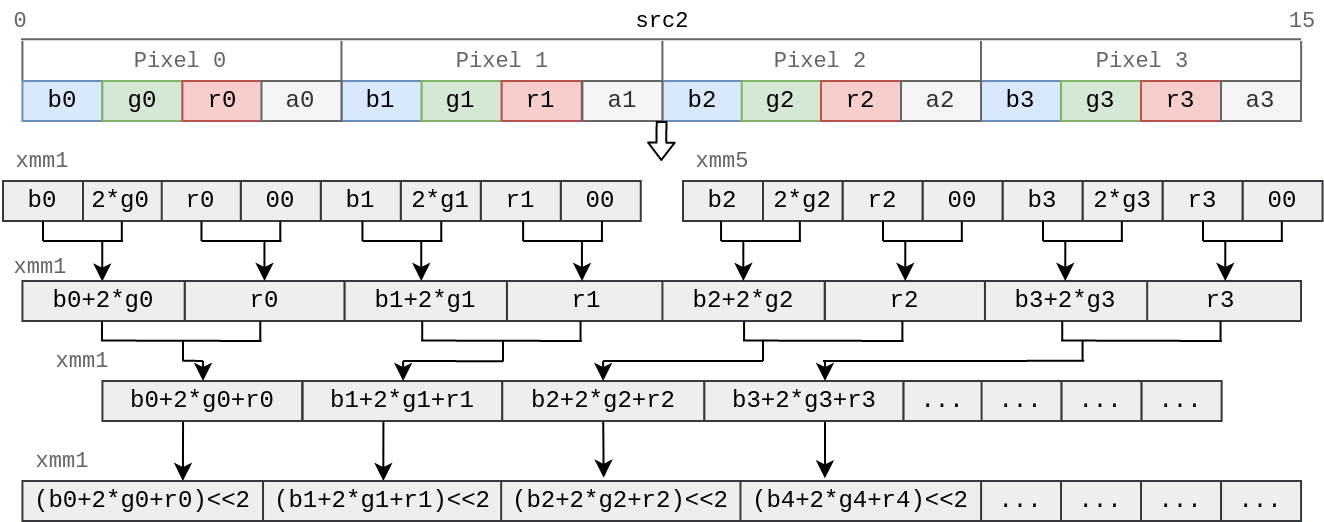
\includegraphics[scale=0.30]{images/filtro-ocultar-1.png}
	\caption{Representación del pasaje de los 4 píxeles contenidos por $src2$ a escala de grises mediante instrucciones de SIMD}
	\label{fig:filtro-ocultar-1}
  \end{center}
\end{figure}

\begin{figure}[h!]
  \begin{center}
	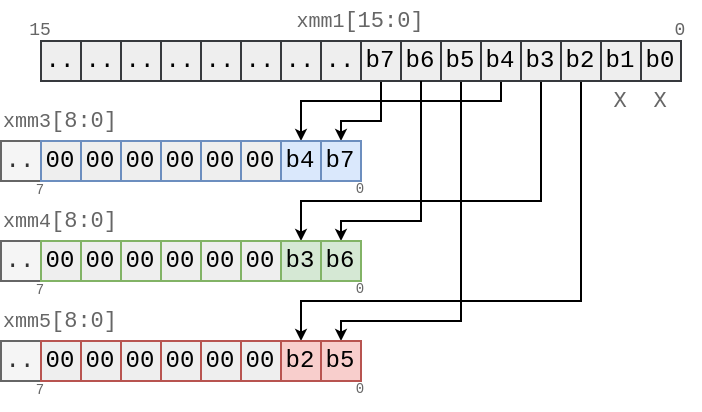
\includegraphics[scale=0.38]{images/filtro-ocultar-2.png}
	\caption{Reordenamiento de los bits $bi$ con $i \in [0,...7]$ para guardar los pixeles en escalas de grises de $src2$ dentro de 3 registros XMM.}
	\label{fig:filtro-ocultar-2}
  \end{center}
\end{figure}

La primer parte del algoritmo, como ya fue anticipado, se trata de convertir los píxeles del $src2$ a píxeles en escala de grises, esto se puede lograr gracias a la formula $(pixel.b + 2*pixel.g + pixel.r)/4$, el cual es la media ponderada de las componentes RGB del píxel.

Para lograr esto se siguen los pasos representados por la Figura \ref{fig:filtro-ocultar-1}, donde en primer lugar se va a levantar el dato del $src2$ y se va a pasar las componentes de $byte$ a $word$ separándolo en dos registros distintos, luego se calcula el doble de la componente $g$ del píxel, después mediante dos sumas horizontales se obtiene la suma $b+2*g+r$ y por ultimo se dividirá el resultado obtenido por $4$ mediante la instrucción de shifteo empaquetado. Nótese que desde la ultima ejecución de la suma horizontal quedo repetida la parte baja de \texttt{xmm1} en su parte alta, pero a fines prácticos sera considerado como basura.

Teniendo los 4 píxeles en blanco y negro se procederá a ejecutar la segunda parte del algoritmo, donde la idea es reorganizar a los bits de cada píxel de la forma retratada en la Figura \ref{fig:filtro-ocultar-2}.
En ella se representa como deben acomodarse los bits individualmente de cada píxel, y se enfoca solamente en lo que sucede con el primer píxel tomado (ya que los otros 3 píxeles harán lo mismo si se usan operaciones de SIMD). Es decir que esta tomando los primeros 16 bits de \texttt{xmm1} (ya que los píxeles contenidos eran del tamaño de una $word$). El procedimiento para llegar a la separación correcta de los bits en los 3 registros XMM correspondientes es mostrado por el algoritmo siguiente, en donde se muestra el pseudocódigo a seguir, pero no así su implementación con instrucciones de SIMD.

\begin{codesnippet}
\begin{verbatim}
    pixel_gs = xmm1[15:0]
    xmm3[8:0] = (((pixel_gs >> 4) & 0x1) << 1) | ((pixel_gs >> 7) & 0x1)
    xmm4[8:0] = (((pixel_gs >> 3) & 0x1) << 1) | ((pixel_gs >> 6) & 0x1)
    xmm5[8:0] = (((pixel_gs >> 2) & 0x1) << 1) | ((pixel_gs >> 5) & 0x1)
\end{verbatim}
\end{codesnippet}

\begin{figure}[h]
  \begin{center}
	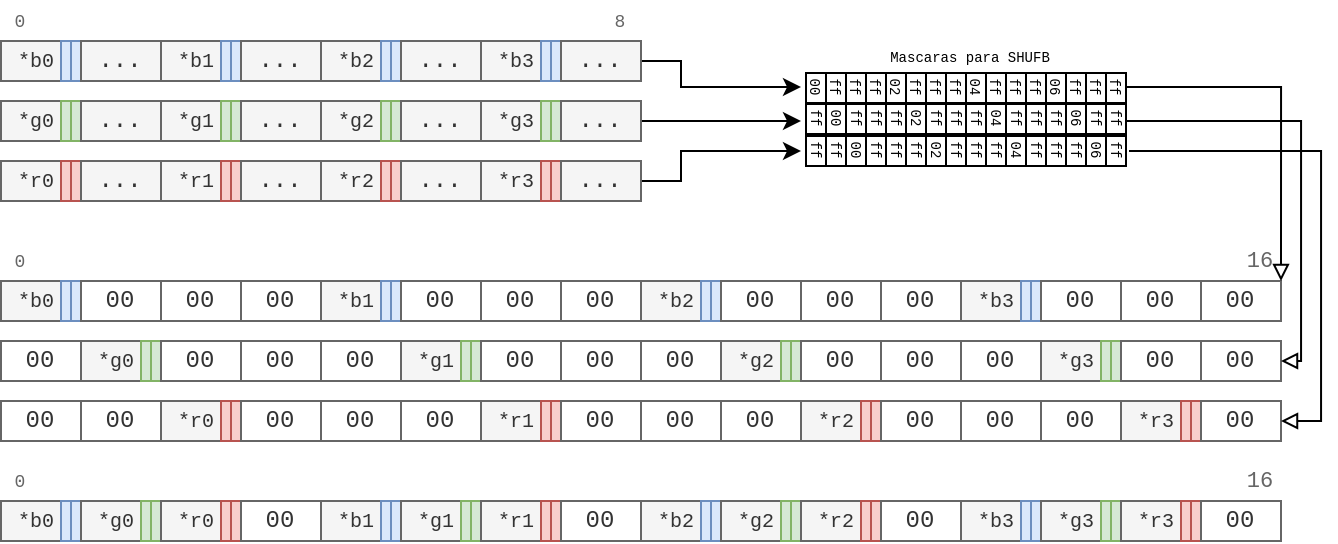
\includegraphics[scale=0.33]{images/filtro-ocultar-3.png}
	\caption{Representación del ordenamiento de los bytes $*bi$ con $i \in [0,...7]$ representados por el color de la componente RGB a la que va a corresponder, mediante mascaras usadas por la instrucción PSHUFB, para luego unir todos los resultados en un solo registro.}
	\label{fig:filtro-ocultar-3}
  \end{center}
\end{figure}

Luego de esto se deben reordenar los píxeles a un solo registro a el mismo orden con el que fueron levantados, esto se refleja en la Figura \ref{fig:filtro-ocultar-3} donde se observa como habían quedado los resultados de las operaciones hechas anteriormente de los registros \texttt{xmm3}, \texttt{xmm4} y \texttt{xmm5}, los cuales cabe destacar que están representados en \emph{Little Endian} solo mostrando la parte baja del registro ya que la parte alta es exactamente igual.
Los 3 registros son pasados por unas mascaras armadas con la finalidad de reacomodar los datos con la instrucción de SSE llamada \texttt{PSHUFB}. Una vez ordenados de la manera correcta se procede a unir los datos a un solo registro mediante la instrucción POR teniendo en cuenta que la componente $alpha$ este seteada en $0$. Por lo tanto hasta este punto ya se ha completado el segundo paso importante del filtro Ocultar.


\begin{figure}[h]
  \begin{center}
	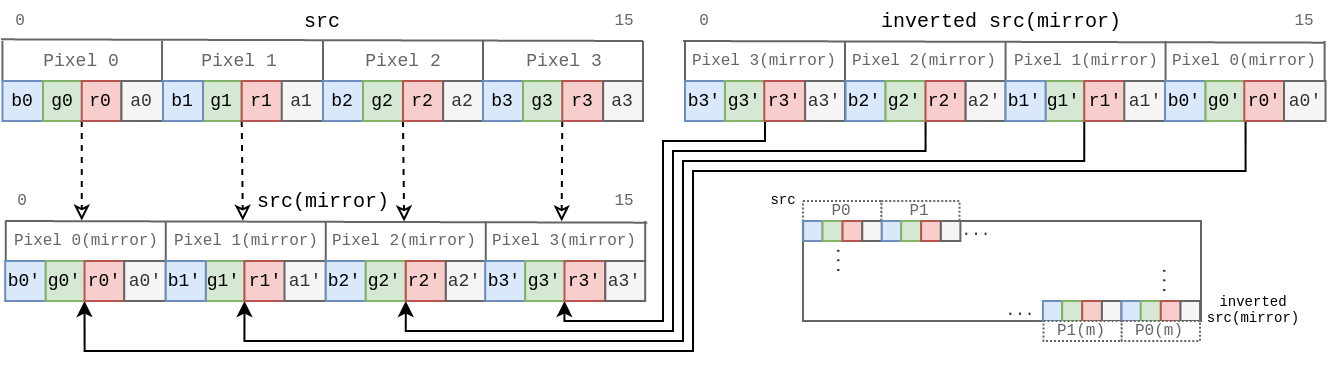
\includegraphics[scale=0.34]{images/filtro-ocultar-4.png}
	\caption{Descripción y obtención del $src(mirror)$ con el diagrama la noción de lo que es un píxel espejo visto como si se tratase de los 2 primeros píxeles de una imagen y sus correspondientes espejos en el extremo opuesto.}
	\label{fig:filtro-ocultar-4}
  \end{center}
\end{figure}

Lo que se procederá a hacer en el ultimo paso de la implementación sera trabajar con el $src(mirror)$ que como se dijo antes serán los píxeles espejos de los que tenga levantadas en un registro XMM del $src$. En la figura \ref{fig:filtro-ocultar-4} se puede observar como se va levanta de memoria a los 4 píxeles de $src$ y los 4 píxeles espejo representados como $inverted\ src(mirror)$ los cuales para trabajar de forma cómoda se los invierte para finalmente tener el $src(mirror)$ que se va a utilizar para obtener el resultado final.

\begin{figure}[h!]
  \begin{center}
	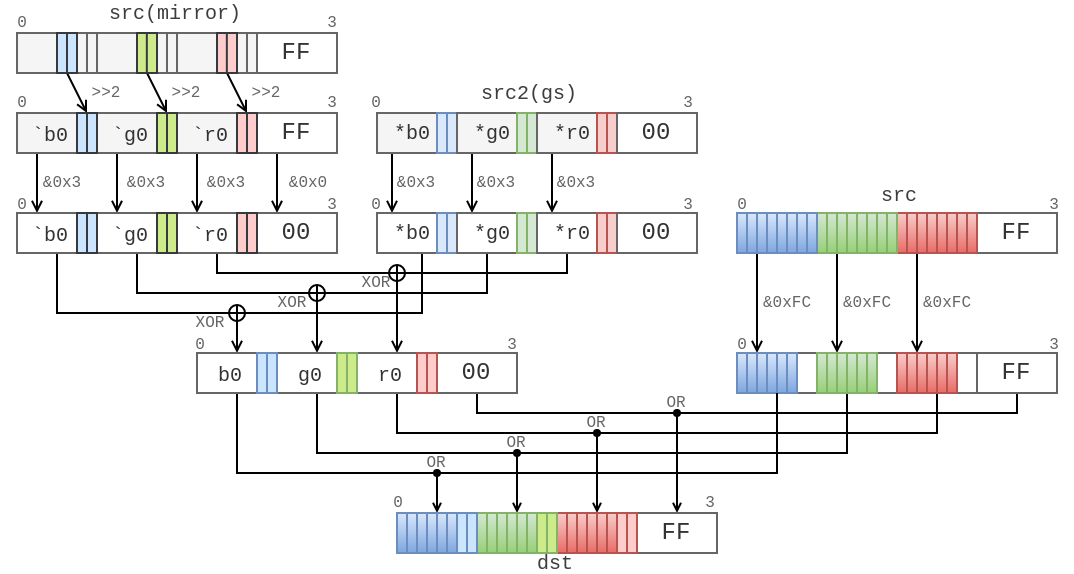
\includegraphics[scale=0.38]{images/filtro-ocultar-5.png}
	\caption{Procesado de los datos obtenidos para poder ser unidos y volcados en la imagen $dst$, representando solo los 4 bytes menos significativos de los registros usados.}
	\label{fig:filtro-ocultar-5}
  \end{center}
\end{figure}

Una vez obtenido el $src(mirror)$ se dan los últimos pasos para obtener el resultado del filtro, la Figura \ref{fig:filtro-ocultar-5} hace el seguimiento de lo que sucede con cada parte obtenida hasta ahora, nótese que solo se muestran los primeros 4 bytes del registro XMM que representa al dato en cuestión.


Se necesita acomodar los bits 2 y 3 del $src(mirror)$ dos lugares a la derecha para mergearlos con los bits obtenidos de en las segunda parte de la implementación, los cuales se muestran en el registro $src2(gs)$ donde $gs$ hace referencia a que se encuentran contenidos en ellos los píxeles en escala de grises (\emph{grey scale}) anteriormente obtenidos. Luego de limpiar los bits que no son necesarios para el resultado de ambos registros además de sus respectivas componentes $alpha$, se mergean el $src(mirror)$ con el $src2(gs)$ mediante la instrucción \texttt{PXOR} que permite que los colores se fundan haciendo así que el cambio no sea fácilmente perceptible por el ojo humano. Por otro lado se debe traer los píxeles de la imagen $src$ cuyos 6 bits mas significativos serán unidos a los dos bits menos significativos del resultado obtenido anteriormente mediante la instrucción \texttt{POR}. Debido a esto se consiguió finalmente lo que se buscaba obtener, los píxeles que se van a guardar en la imagen $dst$ y que tendrá oculta a la imagen $src2$ en escala de grises.



\subsection{Filtro Descubrir}

El filtro Descubrir se encarga de desenmascarar la imagen en escala de grises guardada en los bits 0 y 1 de las componente de cada píxel de la imagen $src$ por el filtro Ocultar visto en la sección \ref{sec:filtro-ocultar}, haciendo los pasos inversos de dicho filtro, y una vez descubiertos serán luego guardados en la imagen $dst$. Cabe resaltar que un píxel en blanco y negro es producto de tener el promedio ponderado del píxel original, en cada una de las componentes RGB del píxel, salvo la componente $alpha$ que debe quedar seteada a \texttt{0xFF}.

Nótese un detalle importante, y es que este filtro trata a todas las imágenes por igual, ya que no sabe si la imagen $src$ contiene realmente una imagen oculta, por lo que la salida de este filtro solo devolverá una imagen en escala de grises significativa si es que se oculto una en el $src$. Dicho esto podemos decir que la ejecución de este filtro solo se reserva para imágenes que hayan pasado por el filtro Ocultar primero, y para el resto de las imágenes en general terminara generando imágenes basura sin ninguna finalidad. El comportamiento de este filtro esta bien representado en la Figura \ref{fig:filtro-descubrir-0}.

\begin{figure}[h!]
  \begin{center}
	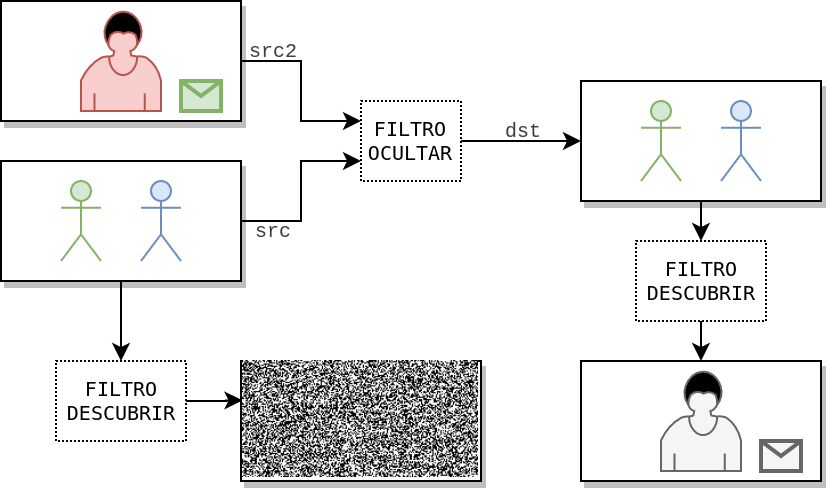
\includegraphics[scale=0.44]{images/filtro-descubrir-0.png}
	\caption{Forma de usar al filtro Descubrir}
	\label{fig:filtro-descubrir-0}
  \end{center}
\end{figure}


\subsubsection{Implementación en ASM}


La implementación del filtro Descubrir es un tanto mas fácil que la del Filtro Ocultar debido a que se debe operar haciendo lo pasos inversos a lo que se realizo en ese filtro. La implementación se dividirá en 3 partes donde primeramente se aislaran los bits que tienen guardada la información de la imagen oculta para ser recuperados por la operación lógica XOR aplicada a esos bits junto a los bits 3 y 4 de cada componente del $src(mirror)$. Luego de obtenerlos se reordenaran los bits obtenidos para poder formar la componente en escala de grises de la imagen oculta. Teniendo la componente se procederá a hacer un broadcast del valor obtenido  hacia las 3 componentes RGB del píxel determinado en la imagen $dst$. Al igual que con el filtro anterior se trabajara con 4 píxeles simultáneamente y cabe destacar que el desarrollo de esta sección sera soportado por imágenes que tal vez no muestren el comportamiento de los 4 píxeles a la vez, y no por esto significa que se deje de operar con los 4 al mismo tiempo ya que siempre se estarán usando instrucciones de SIMD.

\begin{figure}[]
  \begin{center}
	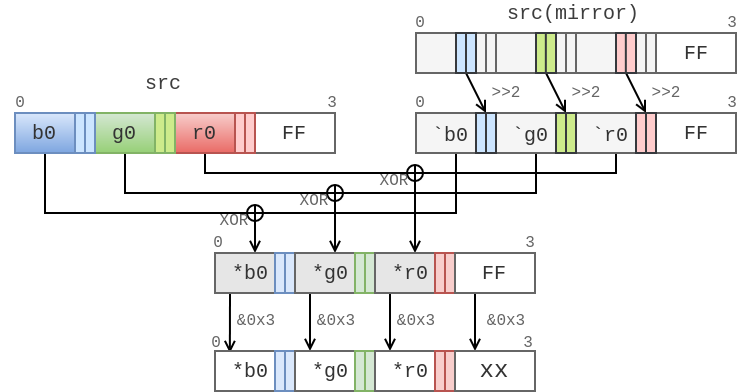
\includegraphics[scale=0.44]{images/filtro-descubrir-1.png}
	\caption{Proceso para recuperar los bits que guardan los valores de los píxeles en escala de grises ocultos, representando las operaciones de SIMD que se utilizan solo en los primeros 4 bytes de los registros usados, siendo representados por las etiquetas $src$ y $src(mirror)$}
	\label{fig:filtro-descubrir-1}
  \end{center}
\end{figure}

La primer parte de la implementación esta representada por la Figura \ref{fig:filtro-descubrir-1} donde ya se supone que se tiene el $src(mirror)$ listo para ser usado (la forma de obtenerlo es igual a la que se presento en la Figura \ref{fig:filtro-ocultar-4} de la sección \ref{sec:filtro-ocultar}). Se shiftea dos bits a derecha a $src(mirror)$, luego junto al $src$ donde se tiene la imagen ingresada, se utiliza la instrucción \texttt{PXOR} la cual devolverá los bits que necesitamos reordenar luego, pero con basura en los bits superiores por lo que se limpiara mediante una mascara con el valor \texttt{0x3} en cada byte, usando la instrucción \texttt{PAND}. Con esto obtenemos los bits que tienen el valor del píxel en escala de grises a desenmascarar.

\begin{figure}[h!]
  \begin{center}
	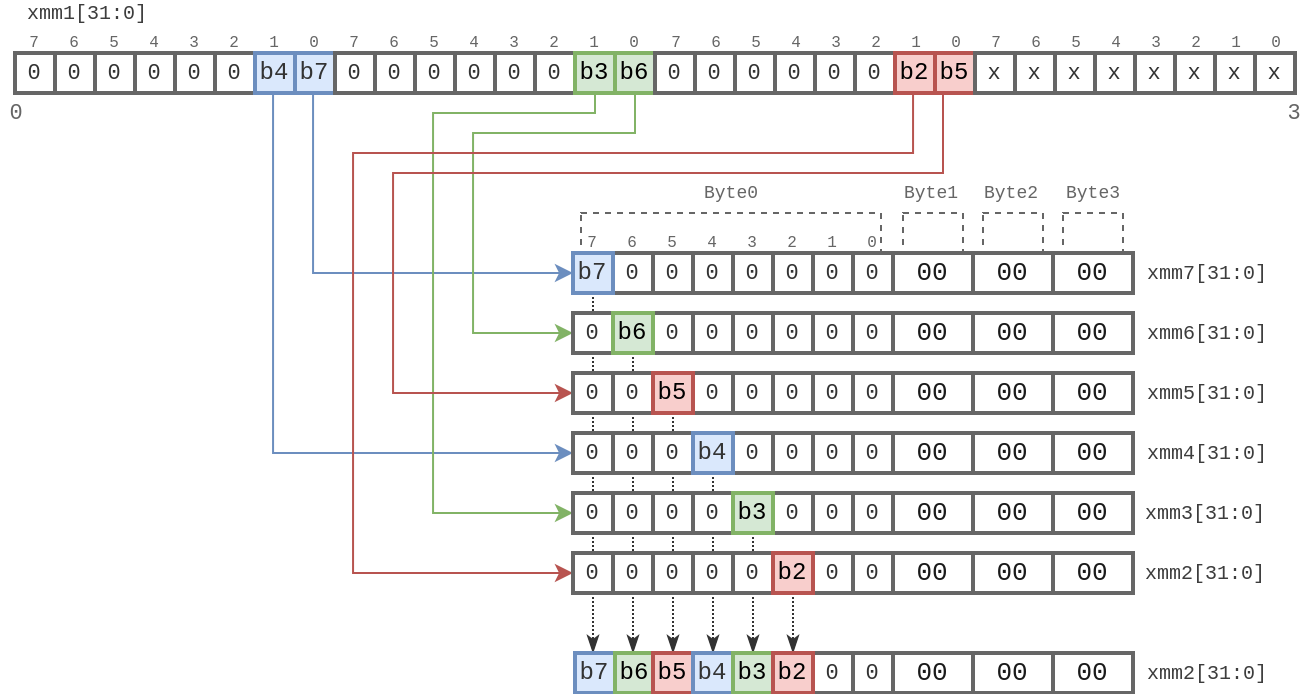
\includegraphics[scale=0.345]{images/filtro-descubrir-2.png}
	\caption{Proceso para obtener los bits acomodados de la forma que se necesita, se divide cada bit en distintos registros para luego ser unidos por la instrucción \texttt{POR}, la cual es usada para unir cada uno de los registros. Con esto se consigue el valor del píxel en escala de grises oculto.}
 	\label{fig:filtro-descubrir-2}
  \end{center}
\end{figure}



La segunda parte del filtro se tratara de reacomodar los bits obtenidos anteriormente de la forma que se explicita en la Figura \ref{fig:filtro-descubrir-2}. Primero se necesita ordenar cada bit individualmente en un registro separado de los demás bits, esto se puede lograr mediante el uso de las instrucciones de shifteo empaquetado, copiando el registro \texttt{xmm1} en registros auxiliares, para conseguir la posición final del bit. Es de destacar que cada bit necesitara un registro aparte solo por la practicidad de luego poder unir los resultados mediante la utilización sucesiva de la operación \texttt{POR}, sin olvidar que en realidad se sigue trabajando con 4 píxeles en simultaneo. Luego de esto se consigue el valor que representa al píxel en escala de grises que estaba oculto en la imagen.

La ultima parte del filtro consiste en formatear a los valores obtenidos en el anterior paso para guardar la imagen que se encontraba oculta en $src$, la Figura \ref{fig:filtro-descubrir-3} hace el seguimiento de los últimos pasos para lograr el dicho cometido.
Se empieza usando una mascara armada para usar la instrucción \texttt{PSHUFB} junto al registro donde se encuentran los valores de los 4 píxeles en escala de grises. Como se dijo anteriormente la forma de imprimir una imagen en escala de grises es hacer un broadcast del valor en las 3 componentes RGB del destino. Por lo que una vez obtenido el registro con los valores de cada píxel en su correspondiente lugar se procede a setear la componente $alpha$ en \texttt{0xFF}. Debido a todo lo hecho hasta este punto ya se puede volcar en memoria el registro XMM con el que estuvimos trabajando, obteniendo en éste los 4 píxeles en escala de grises que se encontraban ocultos.

\begin{figure}[h!]
  \begin{center}
	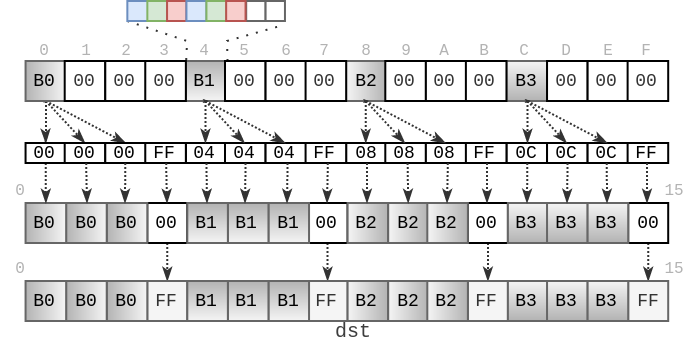
\includegraphics[scale=0.47]{images/filtro-descubrir-3.png}
	\caption{Proceso de broadcast de los bytes donde se encuentra el valor en escala de grises de los píxeles ocultos, mediante una mascara para la instrucción PSHUFB. Y por ultimo el seteado del $alpha$ correspondiente.}
 	\label{fig:filtro-descubrir-3}
  \end{center}
\end{figure}


\newpage

\subsection{Filtro ZigZag}

Un ZigZag es un patrón formado de pequeños renglones de ángulo variable, y constante, trazando un camino entre dos líneas paralelas. Este concepto trasladado a imágenes genera un efecto estético que puede ser descrito como una sensación de movimiento o irregularidad. Esto de logra aplicando operaciones sobre los píxeles de la imagen según la fila en la que se encuentren y colocando un borde blanco de dos píxeles alrededor de la misma. 

Se establece un offset especial para leer y escribir la imagen de origen y destino respectivamente. Se empieza a leer la imagen original desde el primer píxel de la segunda fila, haciendo cuenta de las dos filas de padding que se reservan, pero se empieza a escribir en la imagen final a partir de la segunda columna de la segunda fila.

En el presente desarrollo se utilizaron registros XMM de 128 bits, y dado que cada píxel tiene un tamaño de 32 bits se pueden almacenar hasta 4 píxeles por registro, y por ende este es el total que se puede cargar por acceso a memoria. Con respecto a las iteraciones, en cada fila se hace una sencilla división por 4 para obtener su módulos y poder clasificar las operaciones de acuerdo a 3 casos según la fila i:

\begin{itemize}
\item \textbf{Caso i \% 4 = 1:}
    
Se guarda en la imagen destino los píxeles correspondientes a la imagen original con un offset de dos píxeles a la izquierda. De esta forma se genera el efecto visual de desplazamiento de una tira de la imagen, el cual es característico del ZigZag.

\item \textbf{Caso i \% 4 = 3} 
    
Este caso es análogo al anterior, pero en el sentido opuesto, es decir, se guarda en la imagen destino los píxeles correspondientes a la imagen original con un offset de dos píxeles a la derecha, es decir en el sentido contrario a la fila congruente a 1 modulo 4. 

\item \textbf{Caso i \% 4 = 0 o i \% 4 = 2}

Para las filas pares en este caso se busca suavizar la diferencia entre el desplazamiento de las filas superiores e inferiores mediante un promedio del píxel original y dos adyacentes tanto a izquierda como a derecha por lo que se requieren un total de 5 píxeles por píxel. Esto genera varias dificultades que pueden atentar contra la eficacia de SIMD, por lo cual al considerarse diversas implementaciones surge la interrogante de cual es la mejor. Esto se tratara mas a fondo en la parte de experimentación, pero por ahora se explorará mas a fondo el problema en cuestión. 

Como se menciono anteriormente existe la limitación de 4 píxeles por registro, lo cual es un problema ya que se desea paralelizar las operaciones y ahora en este caso es necesario un segundo acceso a memoria solo por el quinto píxel, sin embargo, se busca procesar múltiples píxeles por iteración por medio de de registros auxiliares de forma que si cargamos en dos accesos a memoria 8 píxeles, estos se trabajen para computar el nuevo valor de 4 píxeles en la imagen destino. Es interesante destacar para el alcance de futuras implementaciones la posibilidad de utilizar registros YMM para solucionar este inconveniente, sin embargo este experimento esta fuera del alcance de este TP en este determinado cuatrimestre.

\end{itemize}

 \begin{figure}[h!]
   \begin{center}
 	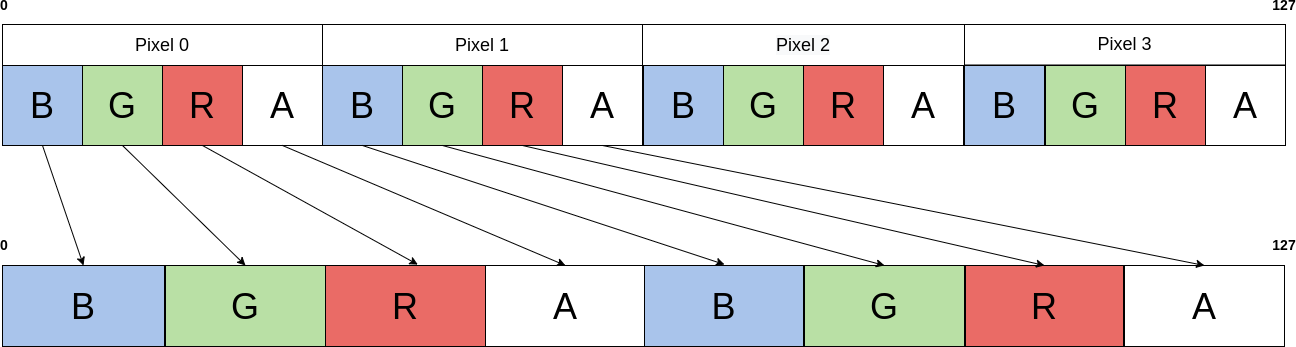
\includegraphics[scale=0.33]{images/filtro-ZigZag-1.jpg}
 	\caption{Extensión de Byte a Word}
 	\label{nombreparareferenciar}
   \end{center}
\end{figure}

Luego, se debe extender cada componente de 8 bits a 16 bits  debido a que la suma de 5 bytes  satura el rango de representación de un byte; evidentemente ahora cada registro puede almacenar un total de 2 píxeles en vez de 4.

\begin{wrapfigure}{r}{5.5cm}
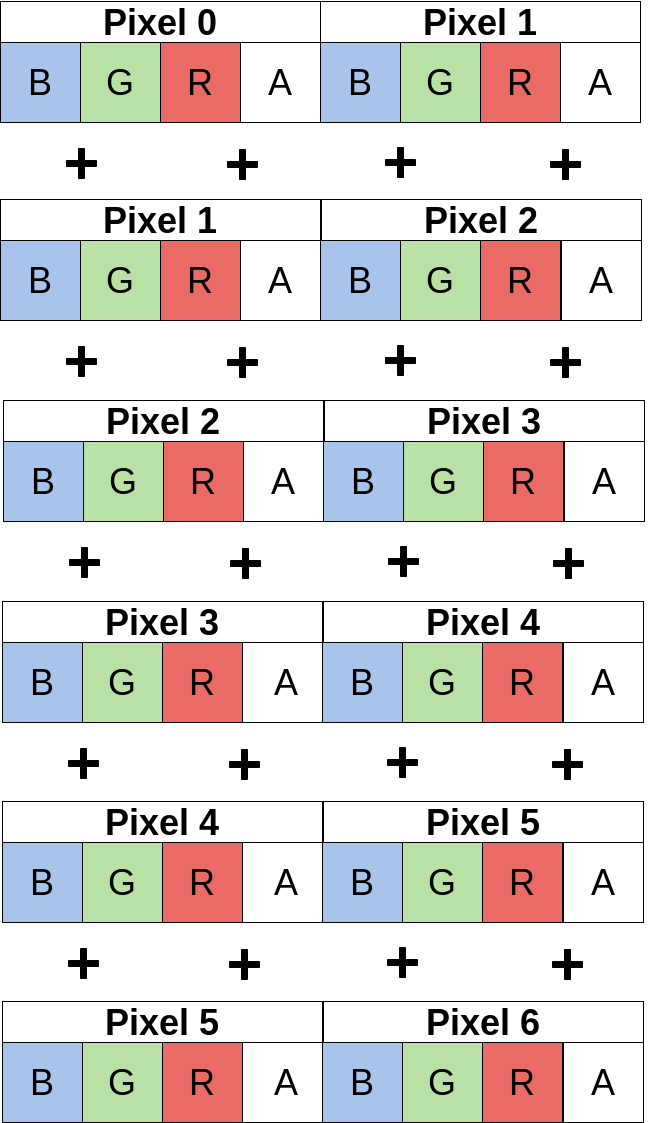
\includegraphics[width=5.5cm]{images/filtro-ZigZag-2.jpg}
\centering
\caption{Suma de píxeles}
\end{wrapfigure}
\par

Ahora es importante destacar que para optimizar el rendimiento se realiza otro acceso a memoria y se cargan 8 píxeles para que una vez realizadas las operaciones se escriban 4 nuevos píxeles ya procesados en la imagen destino.

Se organizan los registros de forma que se ejecute las suma vertical de los 5 píxeles para calcular el promedio. Ahora faltaría dividir por la cantidad de píxeles, es decir, 5 para este filtro.

Es conocido que desde el punto de vista del algoritmo y de la arquitectura del computador que dividir es una operación costosa y que para este set de instrucciones requiere muchos ciclos de clock en comparación a otras operaciones aritméticas. Por otra parte sabemos que la multiplicación de componentes es una función que recibe enteros y devuelve enteros. Mientras que la división de enteros devuelve números reales por lo cual si se quiere utilizar la operación de división se debe trabajar con valores de tipo float. Ya que estos valores de las celdas en memoria se representan como enteros para dividir de la manera tradicional haría falta hacer dos conversiones, primeo de enteros a float, para operar y luego de float a enteros truncando la parte entera de la misma forma que hace el compilador de C. Sin embargo en el presente proyecto se implemento el filtro principal de ZigZag utilizando una técnica que se presume mas eficiente pero menos precisa. Esta diferencia de rendimiento mas adelantes sera evaluada mediante la experimentación para corroborar cual de las 2 técnicas es mejor según el contexto.

Sin embargo, para desarrollar el filtro se debe responder a la incógnita de que N es el correcto o el mejor en este caso dado que el rango de representación se encuentra acotado por 16 bits. El valor elegido en esta ocasión fue $N=8$ y fue encontrado mediante un script de python, entonces el valor a utilizar en la máscara para multiplicar será $51$, que es la parte entera de $2^8/5$ o mejor expresado como $51,2$. Como se menciono anteriormente una vez realizada la multiplicación se toma la parte baja y se shiftea $8$ bits para dividir por $2^8$. Este proceso se aplica para 4 píxeles por iteración, que se guardan en un registro para finalmente hacer una escritura a la imagen de destino. Más detalles de las instrucciones utilizadas a continuación: 

\begin{codesnippet}
\begin{verbatim}
        ; xmm2 = |p2+p3+p4+p5+p6|p1+p2+p3+p4+p5|
        ; xmm0 = |51|51|51|51|51|51|51|
        ...
        pmullw xmm2, xmm0    ; |(p2+p3+p4+p5+p6)*(2^n/5) | (p1+p2+p3+p4+p5+)*(2^n/5)|
        psrlw xmm2, 8        ; |(p2+p3+p4+p5+p6)/5 | (p-2+p-1+p0+p1+p2)/5|
        ...
        packuswb xmm2, xmm11  ; | p3 | p2 | p1 | p0 |
        por xmm2, alfa        ; arreglamos alpha para que siempre valga 255
        movdqu [dest], xmm2
\end{verbatim}
\end{codesnippet}

\newpage
\section{Comparación}
\subsection{Aclaraciones previas}
\begin{itemize}
 \item Nuestra medida de tiempo para los experimentos y las comparaciones será la cantidad de ciclos de ejecución que le tome al procesador realizar la corrida de nuestro programa; éste cuenta con un registro interno, el \textbf{Time Stamp Counter (TSC)}, que lo que hace es incrementar un contador en cada ciclo de ejecución. La Cátedra provee una función que se encarga de invocar a la instrucción en ASM que permite obtener la diferencia de ciclos entre el comienzo y el fin de la ejecución de nuestro programa. No será una medida exacta pero sı́ una buena aproximación debido a que el scheduler del Sistema Operativo puede realizar un cambio de contexto, y además sabiendo que los ciclos no son sólo de nuestro programa.

\item Todos las comparaciones se realizaron en una máquina con un procesador \textbf{Intel Core i7-7700HQ @ 3.800GH} con \textbf{12GB de RAM} y con Ubuntu 18.04.4 como sistema operativo.

\item Para las comparaciones que se detallan, se trató de generar un ambiente en el que no hubiera ``ruido'' proveniente de aplicaciones que pudiéramos estar corriendo, ``matando'' para ello a todos los procesos que pudieran producir algún tipo de alteración. Aun así, y como mencionamos anteriormente, sabemos que el Sistema Operativo constantemente corre procesos que de alguna manera pueden modificar las mediciones.

\item A continuación se comparan las implementaciones desarrolladas en ASM utilizando instrucciones SIMD versus su contra parte en C (versión de la cátedra). Esto se comparara usando dos compiladores distintos, \textbf{GCC y CLANG}, ademas se comparan distintos niveles de optimización del compilador con los flags \textbf{-O0} y \textbf{-O3} a fin de obtener una mayor compresión de el incremento en rendimiento al utilizar operaciones vectoriales. Con respecto a las opciones del compilador se conoce que la versión menos optimizada C-O0 solo mejora el tiempo de compilación y no de ejecución a diferencia de C-03 que si busca optimizar al máximo el rendimiento del programa a ejecutar tanto para GCC como para CLANG, los cuales también serán comparados mas adelante. Se considero representativo correr 500 veces cada filtro y cada una de ellas con un script de Bash con el cual se almacenan la cantidad de ciclos de clock en un .csv para luego interpretar la data y graficar mediante Jupyter Notebooks. 
\end{itemize}

\newpage
\subsection{Filtro Ocultar: C vs ASM}
\subsubsection{Hipótesis}
Siendo un filtro que fue implementado pensando en que corra lo mas eficientemente posible la hipótesis sera que assembler va a ganar por mucho a C con nivel de optimización \textbf{-O0} de CLANG y GCC, ya que además sabemos que la de assembler esta procesando 4 píxeles por iteración frente a la implementación de C que solo procesa un píxel a la vez. Por otro lado se espera que las optimizaciones \textbf{-O3} se acerquen mucho a la implementación de assembler pero que no van a ganar a assembler.

\subsubsection{Resultados}

\begin{figure}[h!]
    \centering
    \subfloat[Muestra de rendimiento de las implementaciones ]{{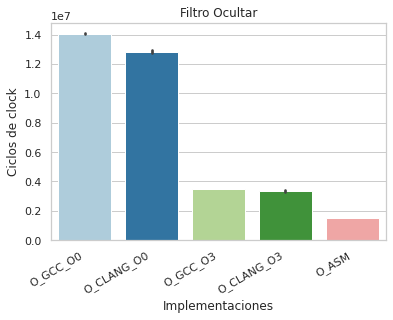
\includegraphics[height=5cm]{graphs/filtro-ocultar-c-vs-asm.png} }}%
    \qquad
    \subfloat[Boxplot de los resultados obtenidos usando ASM ]{{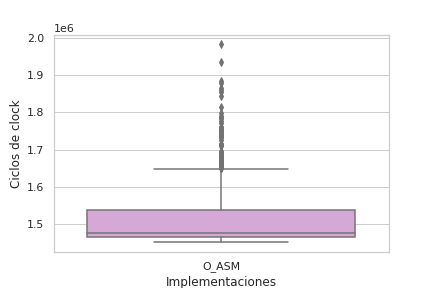
\includegraphics[height=5.5cm]{graphs/filtro-boxplot-ocultar-c-vs-asm-1.png} }}%
    
    \subfloat[Boxplot de los resultados obtenido usandos GCC -O3 ]{{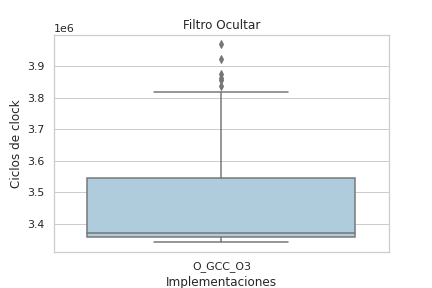
\includegraphics[height=5cm]{graphs/filtro-boxplot-ocultar-c-vs-asm-2.png} }}%
    \qquad
    \subfloat[Boxplot de los resultados obtenido usandos CLANG -O3 ]{{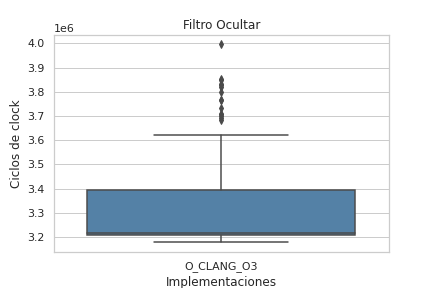
\includegraphics[height=5cm]{graphs/filtro-boxplot-ocultar-c-vs-asm-3.png} }}%
    \caption{Comparaciones entre todas las implementaciones del Filtro Ocultar}
    \label{fig:exp-compare-ocultar}
    
\end{figure}

Como se adelanto en la hipótesis, se puede ver en la Figura \ref{fig:exp-compare-ocultar} que se obtuvo lo que se esperaba. Esto era esperable por el proceso en paralelo que se hace en assembler y por los niveles de optimización de los compiladores. En conclusión se tiene de que el uso de assembler con instrucciones SIMD es mejor opción ante las implementación en C en este filtro.

\newpage 
\subsection{Filtro Descubrir: C vs ASM}
\subsubsection{Hipótesis}
Tenemos muchas similitudes entre el filtro Descubrir y el filtro Ocultar ya que es el encargado de deshacer los cambios del filtro Ocultar, por lo que tiene instrucciones muy similares. Debido a esto se tiene la misma premisa con respecto a lo que se espera con la puesta en prueba del filtro, se espera que tenga un mejor rendimiento frente a la implementación en C del mismo, e incluso frente a las optimización \textbf{-O3} de ambos compiladores.
\subsubsection{Resultados}
\begin{figure}[h!]
    \centering
    \subfloat[Muestra de rendimiento de las implementaciones ]{{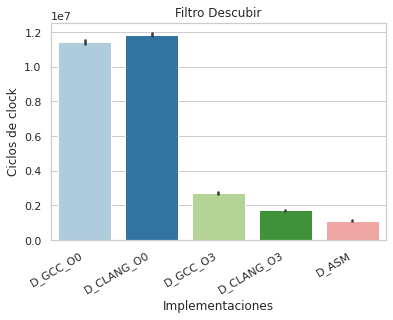
\includegraphics[height=5cm]{graphs/filtro-descubir-c-vs-asm.png} }}%
    \qquad
    \subfloat[Boxplot de los resultados obtenidos usando ASM ]{{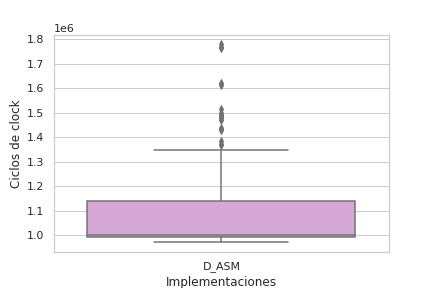
\includegraphics[height=5.5cm]{graphs/filtro-boxplot-descubrir-c-vs-asm-1.png} }}%
    
    \subfloat[Boxplot de los resultados obtenido usandos GCC -O3 ]{{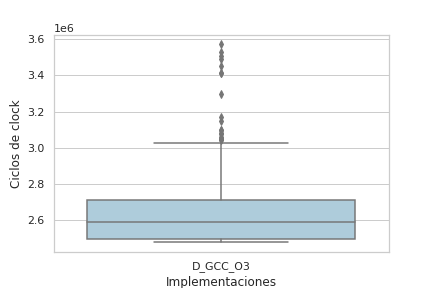
\includegraphics[height=5cm]{graphs/filtro-boxplot-descubrir-c-vs-asm-2.png} }}%
    \qquad
    \subfloat[Boxplot de los resultados obtenido usandos CLANG -O3 ]{{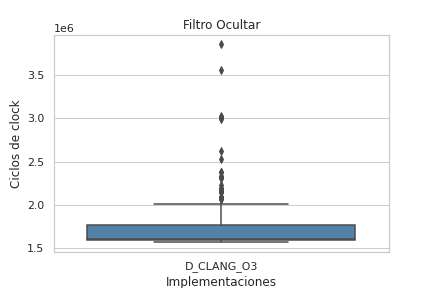
\includegraphics[height=5cm]{graphs/filtro-boxplot-descubrir-c-vs-asm-3.png} }}%
    \caption{Comparaciones entre todas las implementaciones del Filtro Descubrir}
    \label{fig:exp-compare-descubrir}
\end{figure}

Los resultados expresados por la Figura \ref{fig:exp-compare-descubrir} confirman la hipótesis de que ASM con instrucciones SIMD tienen un mejor rendimiento con respecto a las implementaciones de C. Por ultimo cabe destacar el buen rendimiento de la optimización de CLANG -O3 que termino muy cerca de la de ASM.

\newpage
\subsection{Filtro ZigZag: C vs ASM}

\subsubsection{Hipótesis}

Debido a que el filtro de Zigzag está implementado en lenguaje ensamblador y se hace aprovechamiento directo del set de instrucciones \textbf{SSE}, además del hecho de paralelizar las operaciones para procesar hasta 4 píxeles por iteración, se espera por ende que tenga esta implementación un rendimiento muy superior a C en su versión compilada con el flag \textbf{-O0} tanto con CLANG como con CC. Ahora con respecto a la comparación con la versión compilada \textbf{-O3} se espera que el rendimiento siga siendo mayor pero con una diferencia menos significativa debido a la capacidad actual de los compiladores de optimizar código y tiempo de ejecución. 

\subsubsection{Resultados}

\begin{figure}[h!]
    \centering
    \subfloat[Muestra de rendimiento de las implementaciones ]{{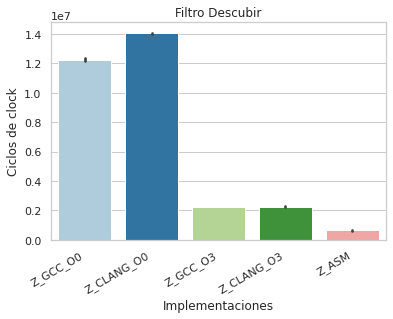
\includegraphics[height=5cm]{graphs/filtro-zigzag-c-vs-asm.png} }}%
    \qquad
    \subfloat[Boxplot de los resultados obtenidos usando ASM ]{{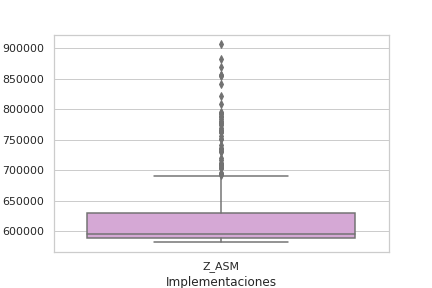
\includegraphics[height=5.5cm]{graphs/filtro-boxplot-zigzag-c-vs-asm-1.png} }}%
    
    \subfloat[Boxplot de los resultados obtenido usandos GCC -O3 ]{{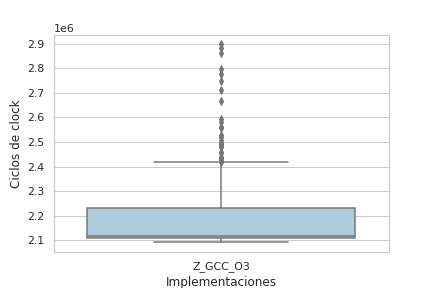
\includegraphics[height=5cm]{graphs/filtro-boxplot-zigzag-c-vs-asm-2.png} }}%
    \qquad
    \subfloat[Boxplot de los resultados obtenido usandos CLANG -O3 ]{{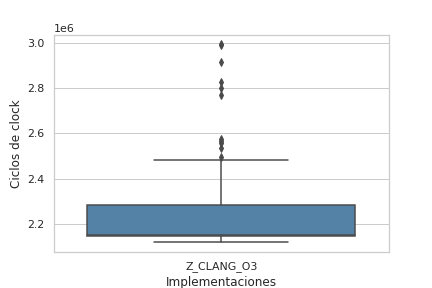
\includegraphics[height=5cm]{graphs/filtro-boxplot-zigzag-c-vs-asm-3.png} }}%
    \caption{Comparaciones entre todas las implementaciones del Filtro ZigZag}
    \label{fig:exp-compare-descubrir}
\end{figure}

Las distribuciones de las comparaciones realizadas se evidencian casi uniformes en los boxplots presentados, con una distancia intercuartil relativamente corta y una cantidad poco representativa de outliers posiblemente generados por interrupciones del sistema operativo. Mediante la experimentación se corroboró la hipótesis planteada, luego de realizar 500 mediciones por caso de estudio se comprobó que la implementación en ASM es la mas eficiente de todas, aunque la versión compilada con el flag -O3 como se esperaba no se queda muy atrás, y para concluir la versión -O3 tuvo un rendimiento mucho peor tanto en GCC como en CLANG, donde este último tuvo el peor rendimiento a diferencia de otros experimentos. Es interesante destacar que la versión de ASM es bastante eficiente ya que se diseño tomando en cuenta las mismas optimizaciones de los compiladores modernos para divisiones por números constantes, y probablemente si se llegase a comparar la implementación en SIMD convirtiendo a floats con la versión de C en su mejor optimización, la diferencia seria mínima o inclusive peor.

\newpage
\section{Experimentos}

Los experimentos serán tomados bajo las mismas condiciones expuestas en la sección anterior, se realizaran 4 experimentos sobre las implementaciones originales en assembly, siendo modificaciones que pueden mejorar, empeorar o no alterar el rendimiento de los algoritmos originales.

\subsection{General: Filtro mas rápido}
Este es un experimento un tanto ingenuo, pero no así deja de ser interesante el saber cual es el algoritmo con mejor rendimiento de entre los 3 filtros ya que, aunque las instrucciones de los filtros Ocultar y Descubrir son un tanto similares, la estrategia necesaria para resolver el filtro de Zigzag es distinta a la de los dos filtros anteriormente mencionados.
Este experimento sera ejecutado por cada filtro 500 veces sobre una imagen de 800x400.
\subsubsection{Hipótesis}
Nuestra hipótesis sera que el filtro Descubrir tendrá mucho mejor rendimiento que los otros filtros debido al menor volumen de instrucciones contenido en su código, sumado a que es un algoritmo relativamente corto.

\subsubsection{Resultados}

 \begin{figure}[h!]
   \begin{center}
 	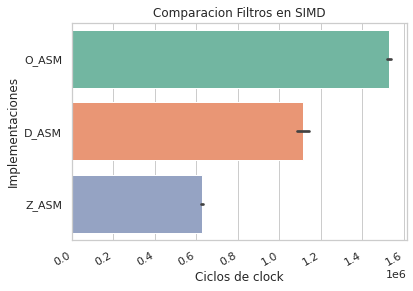
\includegraphics[scale=0.6]{graphs/filtro-comparativo-asm.png}
 	\caption{Comparación entre los filtros implementados en ASM con instrucciones de SSE.}
 	\label{fig:expz-comparativo-asm}
   \end{center}
\end{figure}


Por la Figura \ref{fig:expz-comparativo-asm} podemos ver que no tuvimos el resultado esperado, siendo el filtro Zigzag el que mejor rendimiento tiene. Esto puede ser justificado a la gran optimización que tiene dicho filtro en cuanto a la baja cantidad de operaciones que realiza y a la forma que tiene de dividir dentro de su código (Lo cual sera motivo de otro experimento). Por ultimo se puede agregar que el gráfico deja en claro lo bien optimizados que son los códigos en ASM con instrucciones de SIMD ya que los 3 filtros tienen un muy buen rendimiento.

\newpage

\subsection{Ocultar y Descubrir: Levantando de memoria de forma desalineada}
El no saber si la memoria en la que trabajamos esta alineada o no puede ser un gran problema, esto puede ser comprobado al usar alguna de las instrucciones de SIMD que trabajan levantando memoria, estas producirán errores al momento de ser ejecutadas si es que la memoria no esta alineada, es por esto que es un dato a tener en cuenta cada que vayamos a memoria mientras se trabaja en ASM. Pero por otro lado, ¿que sucede si usamos la instrucción de SSE \texttt{MOVDQU} cada que necesitemos hacer una operación con memoria si sabemos que la memoria esta alineada?. Dicha instrucción levanta y vuelca datos en memoria sin fijarse si está alineada o no. El objetivo de este experimento sera probar si baja considerablemente el rendimiento de los filtros Ocultar y Descubrir al reemplazar los usos de \texttt{MOVDQA} por \texttt{MOVDQU}, donde se harán 500 ejecuciones de ambos filtros sobre una imagen de tamaño 800x400.
\subsubsection{Hipótesis}
La hipótesis que manejaremos sera que el rendimiento de los filtros bajara considerablemente al usar instrucciones para memoria desalineada, siendo que se nos asegura que la memoria está alineada y sabemos que el usar instrucciones de memoria desalineada tiene un costo superior.
\subsubsection{Resultados}
\begin{figure}[h!]
    \begin{center}
 	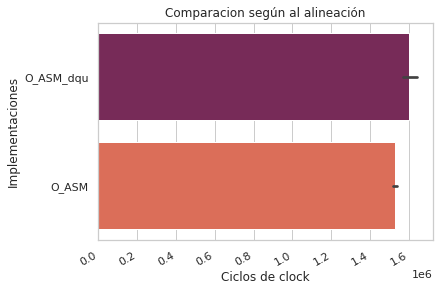
\includegraphics[scale=0.5]{graphs2/filtro-comparativo-O-alineacion-asm.png}
 	\caption{Comparación de rendimiento del filtro Ocultar modificado vs original}
 	\label{fig:exp-ocultar-dqu-vs-dqa}
   \end{center}
    
    \subfloat[]{{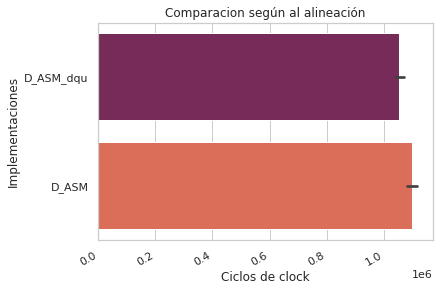
\includegraphics[height=5cm]{graphs2/filtro-comparativo-D-alineacion-asm.png} }}%
    \qquad
    \subfloat[]{{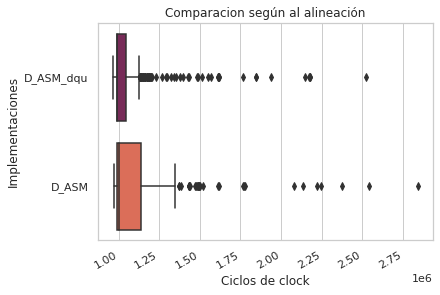
\includegraphics[height=5cm]{graphs2/filtro-comparativo-D-box-alineacion-asm.png} }}%
    \caption{Comparación de rendimiento del Filtro Descubrir modificado vs original}%
    \label{fig:exp-descubrir-dqu-vs-dqa}%
    
\end{figure}

Por parte del filtro Ocultar se vio una diferencia un tanto significativa como muestra la Figura \ref{fig:exp-ocultar-dqu-vs-dqa}, donde se logra ver una ligera reducción de eficiencia al utilizar la instrucción \texttt{MOVDQU}, tal como lo esperábamos.

Y para nuestra sorpresa, con el filtro Descubrir no se cumplió lo esperado según muestra la Figura \ref{fig:exp-descubrir-dqu-vs-dqa} ya que se observa una leve mejora con respecto a la implementación con instrucciones \texttt{MOVDQA}. Podríamos atribuir esto a los outliers que se muestran en el boxplot de la figura \ref{fig:exp-descubrir-dqu-vs-dqa} además del posible ruido del sistema que pudo haber influido en los resultados de este experimento, dado que sabemos que en el peor de los casos el uso de instrucciones \texttt{MOVDQU} no debería ser mejor que el uso de \texttt{MOVDQA} hasta donde sabemos. Consideramos la posibilidad de que la explicación de este comportamiento se encuentre fuera del marco teórico con el que contamos hasta el momento.

\subsection{ZigZag: Dividir con Floats vs Multiplicando}

En el presente experimento se busca comparar principalmente el efecto de dividir multiplicando por un número \emph{mágico} cuando se quiere dividir por una constante, en este caso $2^N/5$ versus convertir los valores a float para operar y luego de vuelta a enteros. Esta ultima operatoria utiliza más instrucciones como se presenta a continuación: 

\begin{codesnippet}
\begin{verbatim}
        ...
        ; xmm2 = |p2+p3+p4+p5+p6|p1+p2+p3+p4+p5| (ENTEROS)
        ;primeros 2 pixeles para dividir (ya son el promedio)
        pmovzxwd xmm10,xmm2  ;|pixel2|pixel1|
        ...
        cvtdq2ps xmm10, xmm10       
        ... 
        divps xmm10, xmm15 ;xmm5 = |5.0|....|5.0|
        ...
        cvttps2dq xmm10, xmm10
        ; de 32 bits a 8 de nuevo (mas instrucciones que al multiplicar por floats)  
        packusdw xmm2, xmm2; | a | r | g | b | a | r | g | b |
        packuswb xmm2, xmm2 ;|a|r|g|b|a|r|g|b|a|r|g|b|a|r|g|b|
       ...
\end{verbatim}
\end{codesnippet}

\subsubsection{Hipótesis}
En vista de que los compiladores modernos utilizan por defecto multiplicar para dividir por constantes, y que el código original tiene menos instrucciones, además de evitar trasladar información dentro del procesador a registros punto flotante, se espera que la versión original sea más rápida y eficiente.

\subsubsection{Resultados}
\begin{figure}[h!]
    \centering
    \subfloat[Escala Lineal ]{{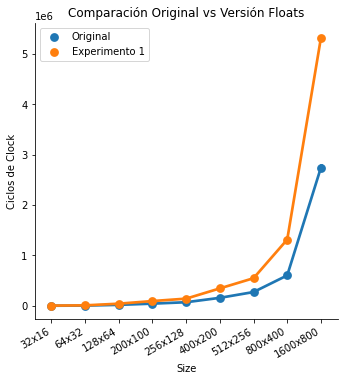
\includegraphics[width=6.5cm]{graphs2/filtro-zigzag-mult-vs-float.png} }}%
    \qquad
    \subfloat[Escala Logarítmica ]{{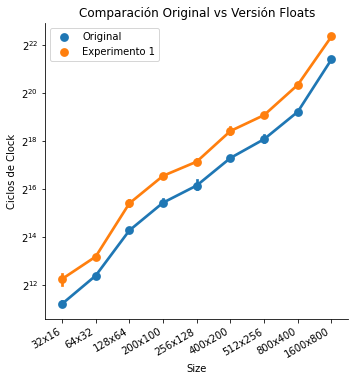
\includegraphics[width=6.5cm]{graphs2/filtro-log-zigzag-mult-vs-float.png} }}%
\end{figure}

En efecto, como se tenia previsto la implementación que hace la conversión resulta menos eficiente que la que divide multiplicando. Esto es debido no solo a que utiliza más instrucciones sino también a que estas son más costosas en comparación a multiplicar o a shiftear que es mucho más barato que dividir. Como se destacaba anteriormente este resultado también se ve influenciado por la micro-arquitectura interna del procesador de Intel que tiene registros específicos para operar con floats a los cuales se debe mover el valor desde otro registro interno (acción implícita en la conversión). Por ultimo se puede apreciar en el gráfico de los resultados del experimento que esta diferencia de eficiencia es casi constante en la escala logarítmica y por ende proporcional en la escala lineal al tamaño de la imagen.


\subsection{ZigZag: Procesando 4 píxeles vs 2 píxeles por iteración}
En este experimento se modificara el código implementado del filtro Zigzag donde se trabajaba con 4 píxeles a la vez, para que este reduzca la cantidad de píxeles trabajados en simultaneo a solo 2.
Se evaluara en una serie de 9 imágenes de tamaño variable: 32x16, 64x32, 128x64, 200x100, 256x128, 400x200, 512x256, 800x400, 1600x800, siendo estos ejecutados 50 veces cada uno para una mejor percepción de los resultados obtenidos.

\subsubsection{Hipótesis}
La hipótesis mas evidente es esperar que el rendimiento sea notablemente afectado por este cambio, dado que se reduce a la mitad la cantidad de píxeles procesados por iteración. Pero no se puede esperar que se dupliquen los valores puesto que como ya se hablo desde el principio del informe, la cantidad de ciclos representados contienen información de procesos no pertinentes al experimento. Lo que si se puede esperar es que haya un incremento (o mejor visto como un step) constante de ciclos con respecto a la implementación original, ya que mínimamente sabemos que se van a duplicar la cantidad de iteraciones realizadas por el algoritmo original de ASM.

\subsubsection{Resultados}
\begin{figure}[h!]
    \centering
    \subfloat[Comparación en escala lineal ]{{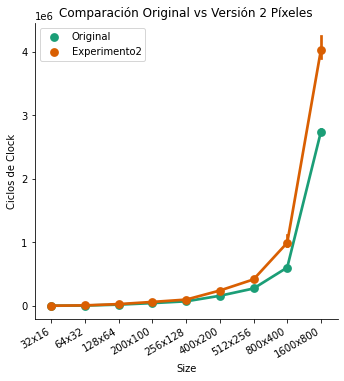
\includegraphics[width=6.5cm]{graphs2/filtro-zigzag-2-vs-4.png} }}%
    \qquad
    \subfloat[Comparación en escala logarítmica ]{{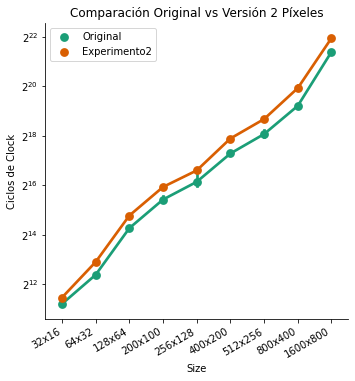
\includegraphics[width=6.5cm]{graphs2/filtro-log-zigzag-2-vs-4.png} }}%
    \caption{Comparación del comportamiento entre la implementación original de Zigzag donde se procesa 4 píxeles en simultaneo contra la implementación donde se procesa 2 píxeles en simultaneo}%
    \label{fig:exp-zigzag-2-pix}%
\end{figure}

Los resultados efectivamente cumplen la hipótesis propuesta ya que como nos muestra la Figura \ref{fig:exp-zigzag-2-pix} los ciclos insumidos por la implementación modificada son notoriamente mayores a medida que crece el tamaño de la imagen que cabe destacar que crecen de forma exponencial, por lo que el verdadero crecimiento se puede ver en la gráfica de escala logarítmica, donde se puede observar el ``step'' mencionado durante la hipótesis, y se comprueba que se mantiene casi constante a medida que crece el tamaño de la imagen. Esto era de esperar por la duplicación de iteraciones que se se lleva a cabo.

\newpage
\section{Conclusiones}

A grandes rasgos podemos concluir que el uso de SIMD es muy beneficioso para este tipo de proyectos en los que se procesan imágenes ya que trabajar en bajo nivel con instrucciones que permiten la manipulación múltiple de datos mejora notoriamente el performance de los filtros así como los tiempo de ejecución. Aunque cabe resaltar que la implementación en ASM es mucho mas costosa en términos de tiempo de desarrollo y planificación que con otros lenguajes de alto nivel y de no ser bien implementada puede traer resultados no esperados e inconvenientes, por lo cual su uso es recomendado en complemento con C para funciones que requieran la mayor eficiencia posible para operaciones vectoriales. Otro desventaja importante a resaltar de la  implementación en SIMD con respecto a los binarios de C es que siempre se debe definir el \emph{target} o usuario final de los filtros ya que algunos procesadores antiguos pero todavía funcionales no son compatibles con este set de instrucciones ya su fabricación es previa a la incorporación de SSE. 

Además en este TP hemos aprendido de que al tratar de medir las ejecuciones de algún algoritmo donde hay que hilar un poco fino, hay factores en una computadora que nos pueden alterar el resultado que esperamos y/o suponemos, ya que tenemos muchísimos programas ejecutándose (fuera de los que matamos) mientras se corren los algoritmos, además de interrupciones al sistema de las cuales no se puede tener un total control. Debido a todo esto las métricas obtenidas podrían no estar mostrando lo que realmente esta pasando, pero dado que no estamos haciendo un benchmarking de nivel profesional, todas estas cuestiones pueden ser tomadas de una forma más relajada, sin dejar de ser crítico a la hora de evaluarlas considerando a  su vez que las magnitudes de los resultados permiten corroborar hipótesis sencillas sobre el comportamiento de los filtros.

También aprendimos hacer un buen tratamiento de los datos durante la etapa de análisis, desde dejar de lado los outliers obtenidos en las distintas mediciones para que las gráficas no se vean afectadas, como también tratar de encontrar respuesta a los sucesos vistos en cada experimento, además del manejo de los datos mediante herramientas externas a la materia para la correcta interpretación y tratamiento de estos.

Queda pendiente para una linea de trabajo futura la realización de experimentos con respecto a aspectos de la cache y los accesos a memoria, además de experimentos relacionados con los saltos condicionales, desenrrollamiento de código.

Dejando de lado el tiempo necesario para poder programar distintos algoritmos con instrucciones de SIMD para ASM, este una buena opción para optimizar distintas estructuras donde se requiera de un paralelismo básico para acelerar su ejecución, ya sea en las áreas de manipulación de datos multimedia, así como en criptografía y relacionadas. 

Hoy en día SSE es una excelente alternativa para el desarrollo de funciones eficientes y robustas en total control de las capacidades del procesador Intel, finalmente queda la expectativa de que nuevas sorpresas o sets de instrucciones serán incorporadas en los procesadores del futuro. 


%¿Cuál implementación es “mejor”?
%¿Qué métricas se pueden utilizar para calificar las implementaciones y cuantificarlas?
%¿En qué casos? ¿De qué depende? ¿Depende del tamaño de la imagen? ¿Depende de la imagenen sı́? ¿De los parámetros?
%¿Cómo se podrı́an mejorar las métricas de las implementaciones propuestas? ¿Cuáles no se pueden mejorar?
%¿Es una comparación justa? ¿De qué depende la velocidad del código C? ¿Cómo puede optimizarse?
%¿Cuál es la cantidad de instrucciones ejecutadas por pı́xel en cada implementación? ¿Y de accesos a memoria? ¿Se condice empı́ricamente esta diferencia en la performance de los filtros?
%¿Hay diferencias en operar con enteros o punto flotante? ¿La imagen final tiene diferencias significativas?
%¿El overhead de llamados a funciones es significativo? ¿Se puede medir?
%¿Las limitaciones de performance son causadas por los accesos a memoria? ¿O a la memoria cache? ¿Se podrı́a acceder mejor a esta?
%¿Y los saltos condicionales? ¿Afectan la performance? ¿Es posible evitarlos total o parcialmente?
%¿El patrón de acceso a la memoria es desalineado? ¿Hay forma de mejorarlo? ¿Es posible medir cuánto se pierde?

\end{document}

